81. $g(x)=\cfrac{x-2}{2x-x^2}=\cfrac{x-2}{x(2-x)}=-\cfrac{1}{x},\ x\neq2.$
$$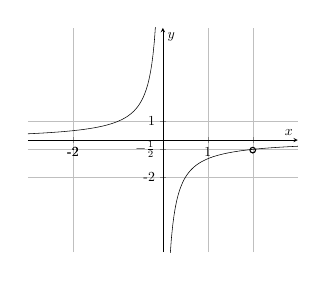
\begin{tikzpicture}[scale=0.5]
\begin{axis}[
    axis lines = middle,
    grid=major,
    legend pos={south west},
    xlabel = {$x$},
    %xlabel style={below right},
    ylabel = {$y$},
    ymin=-6,
    ymax=6,
    xmin=-3,
    xmax=3,
    xtick={-2, -2,  1, 2},
    xticklabels={-2, -2, 1, $ $},
    ytick={-2,-0.5, 1},
    yticklabels={-2,$-\frac{1}{2}$, 1},
                  ]
	\addplot[domain=-3:-0.1, samples=100, color=black] {-1/x};
    \addplot[domain=0.1:3, samples=100, color=black] {-1/x};
        %\addplot[domain=2.01:6, samples=100, color=black] {2/(2-x)};
   % \addplot[domain=-3:3, samples=100, color=black] {-x};
     %\addlegendentry{$\text{Рис. 1}$};
\end{axis}
\draw (5.71,2.59) circle (2pt);
%\draw (3.45,0.75) circle (2pt);
%\draw (3.45,2.55) circle (2pt);
\end{tikzpicture}$$
а) Прямая $y=kx$ имеет с графиком $g(x)$ одну общую точку, если проходит через точку $\left(2;-\cfrac{1}{2}\right),$ то есть если $2k=-\cfrac{1}{2},\ k=-\cfrac{1}{4}.$\\
б) Для нахождения общих точек графика и прямой, составим уравнение $-\cfrac{1}{x}=bx+2,\ bx^2+2x+1=0,$ при этом $x\neq2.$ Это уравнение имеет один корень либо при $b=0$ $\left(\text{тогда }x=-\cfrac{1}{2}\right),$ либо при $\cfrac{D}{4}=1-b=0,\ b=1\ \left(\text{тогда }x=-1\right),$ либо если одним из корней является $x=2,$ то есть $b\cdot4+4+1=0,\ b=-\cfrac{5}{4}.$\\
